\documentclass[12pt,a4paper,preprint,nopreprintline]{elsarticle}

\usepackage[T1]{fontenc}
\usepackage[utf8]{inputenc}
\usepackage[english]{babel}
\usepackage{amsmath,amssymb,amsfonts,bm}
\usepackage{graphicx}
\usepackage{booktabs}
\usepackage{multirow}
\usepackage{array}
\usepackage{tabularx}
\usepackage{xcolor}
\usepackage{hyperref}
\graphicspath{{figs/}}

\usepackage[
    a4paper,
    left=2cm,
    right=2cm,
    top=2cm,
    bottom=2.7cm
]{geometry}

\makeatletter
\setlength{\@fptop}{0pt}
\setlength{\@fpsep}{8pt}
\setlength{\@fpbot}{0pt plus 1fil}
\makeatother
\setlength{\abovecaptionskip}{4pt}
\setlength{\belowcaptionskip}{2pt}
\renewcommand{\floatpagefraction}{0.05}

\hyphenation{Schwarz-schild Lich-ne-ro-wicz baro-clinic}

\begin{document}
\makeatletter
\setlength{\@fptop}{0pt}%
\setlength{\@fpsep}{8pt}%
\setlength{\@fpbot}{0pt plus 1fil}%
\makeatother

\begin{frontmatter}

\title{Perturbation Spectrum of Michel Flow:\\
Acoustic, Vortical, and Entropy Modes}

\author{Alexander V. Semyannikov}
\ead{avsemyannikov@gmail.com}
\address{Independent Researcher}

\begin{abstract}
We study the spectrum of linear perturbations of relativistic spherical accretion onto a Schwarzschild black hole (Michel flow), carrying the Newtonian analysis of the spatial stability of Bondi accretion over to full general relativity. Small perturbations of a perfect fluid split into three families -- acoustic, vortical, and entropy modes -- which we treat together in the language of acoustic geometry. The acoustic sector reduces to a one-dimensional Schr\"odinger-type equation with an explicit effective potential: it recovers the standard scalar Schwarzschild potential in the vacuum limit and the known Newtonian wave equation of Bondi flow in the nonrelativistic limit. For a transonic Michel background the sonic point coincides exactly with the acoustic horizon, and a Frobenius analysis shows that this horizon replaces the Newtonian central endpoint: the non-trivial radial exponent is purely imaginary, so the local solutions are travelling waves rather than growing powers. Our main result is that the acoustic horizon regularizes the exterior spatial problem. The Newtonian non-radial instability, which operates for $\gamma<5/3$, relies on growth towards a point-mass endpoint; the exterior Michel domain has no such endpoint -- the relative amplitudes of all three sectors approach finite values at the horizon -- and the supersonic shell is causally disconnected from it. Vortical and entropy perturbations are advected invariants with a single ingoing characteristic: frozen into the flow, they are carried through the horizon, and the entropy mode additionally sources sound and vorticity through a relativistic baroclinic term. Numerical integration of the scattering problem confirms flux conservation and the absence of superradiance. The externally accessible flow is therefore free of the Newtonian central power-law instability.
\end{abstract}

\begin{keyword}
Michel accretion \sep relativistic hydrodynamics \sep acoustic perturbations \sep vortical modes \sep entropy modes \sep spatial stability \sep acoustic horizon
\end{keyword}

\end{frontmatter}

\section{Introduction}
\label{sec:introduction}

Steady spherical accretion provides a minimal setting in which gravity, compressible flow, and wave propagation can be studied together. Its Newtonian form is the Bondi solution~\cite{BondiH_OnSphericallySymmetricalAccretion_1953}, while the relativistic flow onto a Schwarzschild black hole is described by the Michel solution~\cite{MichelFC_AccretionOfMatterByCondensedObjects_1972}. The transonic background possesses an acoustic horizon that controls the propagation of linear acoustic disturbances and gives rise to an effective relativistic acoustic geometry~\cite{MoncriefV_StabilityOfStationarySphericalAccretionOntoASchwarzschildBlackHole_1980,BilicN_RelativisticAcousticGeometry_1999}.

The stability of steady spherical accretion has a long history. In the Newtonian setting, Bondi flow was shown to be stable against radial perturbations~\cite{GarlickAR_TheStabilityOfBondiAccretion_1979,PettersonJA_SilkJ_OstrikerJP_VariationsOnAShpericallySymmetricalAccretionFlow_1980}, while Ref.~\cite{KovalenkoIG_EreminMA_SpatialInstabilityOfSphericalAccretion_1998} recast the problem as one of \emph{spatial} stability and found that non-radial perturbations of all three fluid mode families grow towards the accretor for $\gamma<5/3$. In shocked flows the advective-acoustic cycle couples entropy and vorticity to sound and can drive a genuine instability~\cite{FoglizzoT_TaggerM_EntropicAcousticInstabilityInShockedAccretionFlows_2000,FoglizzoT_EntropicAcousticInstabilityOfShockedBondiAccretionIWhatDoesPerturbedBondiAccretionSoundLike_2000}. In the relativistic Michel flow, in turn, potential (acoustic) perturbations were shown to be stable and to form a quasi-normal spectrum controlled by the acoustic horizon~\cite{MoncriefV_StabilityOfStationarySphericalAccretionOntoASchwarzschildBlackHole_1980,ChaverraE_MoralesMD_SarbachO_QuasinormalAcousticOscillationsInTheMichelFlow_2015}.

These strands have not been combined: the relativistic analyses treat only the acoustic (potential) sector, whereas the full spatial-stability problem for all three mode families has been solved only in the Newtonian, shock-free case. A general perturbation of a perfect fluid also carries vorticity and entropy degrees of freedom, which are advected by the background flow and can source the acoustic response. The present paper closes this gap by carrying the Newtonian spatial-stability analysis~\cite{KovalenkoIG_EreminMA_SpatialInstabilityOfSphericalAccretion_1998} over to the relativistic Michel flow, for the acoustic, vortical, and entropy sectors together.

The causal geometry of this background and the high-frequency dynamics of its sound rays were developed in a companion study~\cite{SemyannikovAV_AcousticGeometryAndSoundRayDynamics_2026}. The present work uses the same Michel background and normalization, but moves beyond the geometric-optics limit to the full finite-frequency perturbation system, including the degrees of freedom that do not propagate on the acoustic null cone. From the companion paper we import the acoustic metric and the Michel integrals; the sonic-point conditions and the identification $r_{\mathrm{a}}=r_{\mathrm{c}}$ are restated in Sec.~\ref{sec:michel_background} for later use.

This paper develops a common description of all three mode families. In particular, we:
\begin{itemize}
    \item derive the linearized continuity, Euler (vorticity form), and entropy-advection equations on the Michel background and classify the acoustic, vortical, and entropy sectors;
    \item reduce the acoustic sector to a one-dimensional Schr\"odinger-type equation and validate it against the scalar Schwarzschild and Newtonian limits;
    \item show that the sonic point coincides with the acoustic horizon and that the horizon replaces the Newtonian central endpoint, with a purely imaginary non-trivial Frobenius exponent;
    \item establish the central result that the acoustic horizon regularizes the externally accessible spatial problem and removes the central power-law mechanism of the Newtonian non-radial instability;
    \item extend the argument to the advected vortical and entropy sectors and to the baroclinic coupling by which entropy sources sound and vorticity, recovering the Bondi limit in each case;
    \item confirm stability numerically through the acoustic scattering problem (flux conservation, absence of superradiance).
\end{itemize}

The paper is organized as follows. Section~\ref{sec:background} summarizes the Michel background and derives the full linear perturbation system with its mode classification. Each of the three families is then treated along the same lines: the equations on the Michel background, their asymptotics at the acoustic horizon, the Newtonian limit, and the Bondi-flow asymptotics that follow from it. This pattern is followed by Sec.~\ref{sec:acoustic} (acoustic modes, including horizon regularization of the exterior problem and acoustic scattering), Sec.~\ref{sec:vortical} (vortical modes), and Sec.~\ref{sec:entropy} (entropy modes and the baroclinic coupling between sectors). Section~\ref{sec:discussion} combines the three sectors into a unified spectrum, and Section~\ref{sec:conclusions} summarizes the results.

\section{Michel background and linear perturbation system}
\label{sec:background}

\subsection{Conventions and stationary transonic flow}
\label{sec:michel_background}

We adopt the metric signature $\mathfrak{s}=(-,+,+,+)$ and work throughout with dimensionless variables: lengths are measured in units of the gravitational radius $r_{\mathrm{g}}=2GM/c^{2}$, velocities and the sound speed in units of $c$, and the thermodynamic variables on their asymptotic rest-frame scales, as is standard for Michel flow~\cite{MichelFC_AccretionOfMatterByCondensedObjects_1972,MoncriefV_StabilityOfStationarySphericalAccretionOntoASchwarzschildBlackHole_1980}. The Schwarzschild line element then reads
\begin{equation}
    \mathrm{d}s^{2}
    =
    -f\,\mathrm{d}t^{2}
    +f^{-1}\,\mathrm{d}r^{2}
    +r^{2}\left(
        \mathrm{d}\theta^{2}
        +\sin^{2}\theta\,\mathrm{d}\phi^{2}
    \right),
    \qquad
    f(r)=1-\frac{1}{r}.
    \label{eq:schwarzschild_metric}
\end{equation}
with the event horizon at $r=1$. A stationary, spherically symmetric flow carries the 4-velocity
\begin{equation}
    u^{\mu}=(\vartheta,\upsilon,0,0),
    \qquad
    f\vartheta=\sqrt{f+\upsilon^{2}},
    \qquad
    \upsilon<0,
    \label{eq:background_velocity}
\end{equation}
where the relation between $\vartheta$ and $\upsilon$ follows from the normalization
\begin{equation}
    u_{\mu}u^{\mu}=-1,
    \label{eq:four_velocity_normalization}
\end{equation}
while $\upsilon<0$ describes inward motion and thus selects the accretion branch.

The medium is a perfect fluid with baryon number density $n$, energy density $\epsilon$, pressure $p$, and specific enthalpy $h$, related by
\begin{equation}
    h=\frac{\epsilon+p}{n},
    \qquad
    a^{2}=
    \left(\frac{\partial p}{\partial\epsilon}\right)_{S}=
    \frac{1}{h}\left(\frac{\partial p}{\partial n}\right)_{S},
    \label{eq:enthalpy_sound_speed}
\end{equation}
where $a$ is the local sound speed in units of $c$. The equation of state is taken to be polytropic,
\begin{equation}
    p=K(S)n^{\gamma},
    \qquad
    h=\frac{\gamma-1}{\gamma-1-a^{2}}.
    \label{eq:polytropic_closure}
\end{equation}
A homentropic Michel solution is thus fixed by the adiabatic index $\gamma$ and the asymptotic sound speed $a_{\infty}$.

Two first integrals suffice to close the background. Baryon conservation and the relativistic Bernoulli relation,
\begin{equation}
    r^{2}n\upsilon=\mathcal{J},
    \qquad
    h\sqrt{f+\upsilon^{2}}=
    \frac{\gamma-1}{\gamma-1-a_{\infty}^{2}}=
    h_{\infty},
    \label{eq:michel_integrals}
\end{equation}
where $\mathcal{J}<0$ is the conserved inward baryon flux, whose sign follows from $\upsilon<0$, and $h_{\infty}$ is the specific enthalpy at spatial infinity. Together with the equation of state, these relations determine the profiles $\upsilon(r)$, $a(r)$, and $n(r)$ once the pair $(\gamma,a_{\infty})$ is chosen~\cite{MichelFC_AccretionOfMatterByCondensedObjects_1972}.

A smooth transition through the sonic point requires the numerator and denominator of $\mathrm{d}\upsilon/\mathrm{d}r$ to vanish together at a single radius $r=r_{\mathrm{c}}$, which yields the critical-point conditions
\begin{equation}
    \upsilon_{\mathrm{c}}^{2}=\frac{1}{4r_{\mathrm{c}}},
    \qquad
    a_{\mathrm{c}}^{2}=
    \frac{1}{4r_{\mathrm{c}}-3}=
    \frac{\upsilon_{\mathrm{c}}^{2}}{1-3\upsilon_{\mathrm{c}}^{2}}.
    \label{eq:sonic_conditions}
\end{equation}
Linear acoustic disturbances of this flow do not propagate on the Schwarzschild metric but on an effective acoustic geometry~\cite{SemyannikovAV_AcousticGeometryAndSoundRayDynamics_2026,VisserM_AcousticBlackHolesHorizonsErgospheresAndHawkingRadiation_1998,BilicN_RelativisticAcousticGeometry_1999}, whose contravariant core is
\begin{equation}
    \eta^{\mu\nu}
    =
    g^{\mu\nu}+\left(1-a^{-2}\right)u^{\mu}u^{\nu} .
    \label{eq:acoustic_core}
\end{equation}
The acoustic horizon $r=r_{\mathrm{a}}$, defined by $\eta^{rr}(r_{\mathrm{a}})=0$, coincides with the sonic critical point, $r_{\mathrm{a}}=r_{\mathrm{c}}$, as shown in~\cite{SemyannikovAV_AcousticGeometryAndSoundRayDynamics_2026}. The supersonic shell $1<r<r_{\mathrm{a}}$ therefore sits inside the acoustic horizon. For cold asymptotic gas ($a_{\infty}\ll1$) the horizon lies far out in the Newtonian region, $r_{\mathrm{a}}\sim a_{\infty}^{-2}\gg1$, and migrates towards the black hole as $a_{\infty}$ grows. As the surface past which no acoustic signal can return, it sets the natural inner boundary of the perturbation problem to which we now turn. The causal structure that fixes this boundary is shown in Fig.~\ref{fig:causal_structure}(b); the same structure governs the advective sectors, whose characteristic is the fluid worldline itself. The Newtonian picture in Fig.~\ref{fig:causal_structure}(a) differs only in its inner end: an acoustic horizon exists there as well, but behind it lies the point mass itself, which both sound and fluid reach in finite time.

\begin{figure}[!tb]
\centering
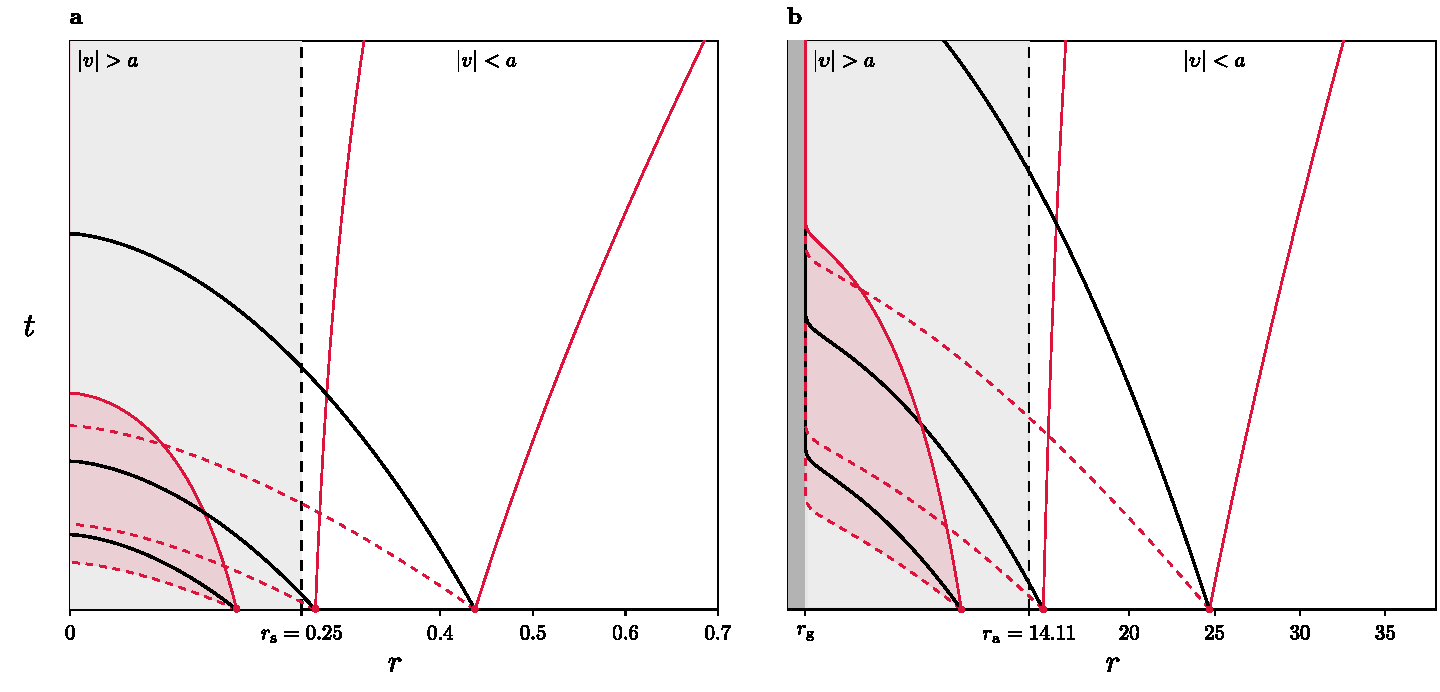
\includegraphics[width=0.98\linewidth]{causal_structure.pdf}
\caption{Causal structure of the two flows in the $(r,t)$ plane; time increases upward, with its own scale in each panel. (a)~Newtonian Bondi flow in absolute time ($r_{\mathrm{s}}=0.25\,r_{\mathrm{B}}$). (b)~Michel flow in Schwarzschild coordinates at $a_{\infty}=0.1$ ($r_{\mathrm{a}}=14.11\,r_{\mathrm{g}}$), the same background as in panel~(b) of Fig.~\ref{fig:mach_topology}. Both flows are taken at $\gamma=4/3$: the value $5/3$ is of no use here, since the Bondi sonic point then runs into the centre. The crimson dots are the emission events: in panel~(a) they sit at $r=0.18$, $0.27$ and $0.44\,r_{\mathrm{B}}$, in panel~(b) at $r=10.2$, $15.0$ and $24.7\,r_{\mathrm{g}}$. In both flows these are the same fractions of the acoustic horizon radius, $0.72$, $1.06$ and $1.75$; the radii themselves differ only because the horizons do, $r_{\mathrm{s}}=0.25\,r_{\mathrm{B}}$ for Bondi against $r_{\mathrm{a}}=14.11\,r_{\mathrm{g}}$ for Michel. From each event both sound characteristics are emitted: solid crimson is the outgoing branch, dashed the ingoing one; black curves are the fluid worldlines, the single characteristic of the invariants $\delta\omega_{\mu\nu}$ and $\delta S$. The characteristic velocities are given by Eq.~\eqref{eq:acoustic_surface_gravity} for Michel flow and by the plain sum $v_{\pm}=v\pm a$ for Bondi flow. The grey band is the supersonic shell and the vertical dashed line the acoustic horizon, where $v_{+}=0$: inside the shell both sound branches point inward and the region of influence of an event (shading) never leaves the horizon, while outside the outgoing branch escapes but freezes linearly in the distance to the horizon. This freezing is the same in both flows and produces the same logarithmic stretching set by the surface gravity $\kappa$. What differs is the inner end. For Bondi flow the point mass itself stands behind the acoustic horizon, and the sound rays together with the fluid worldlines reach $r=0$ in finite time. For Michel flow the inner end is the gravitational horizon (dark band): the turn of the curves towards the vertical as $r\rightarrow r_{\mathrm{g}}$ is the Schwarzschild coordinate singularity rather than a physical freezing, but it is precisely what makes the coordinate infall time infinite. Replacing the point mass by a black hole removes the inner boundary along with it.}
\label{fig:causal_structure}
\end{figure}

\subsection{Linearized hydrodynamic equations}
\label{sec:linearized_system}

The dynamics of an ideal relativistic fluid is governed by particle conservation, the Lich\-ne\-ro\-wicz--Crocco form of the Euler equation, and entropy advection,
\begin{equation}
    \nabla_{\mu}(nu^{\mu})=0,
    \label{eq:continuity}
\end{equation}
\begin{equation}
    u^{\mu}\omega_{\mu\nu}=T\,\partial_{\nu}S,
    \label{eq:euler_crocco}
\end{equation}
\begin{equation}
    \omega_{\mu\nu}
    \equiv
    \partial_{\mu}(hu_{\nu})-\partial_{\nu}(hu_{\mu}),
    \label{eq:vorticity_definition}
\end{equation}
\begin{equation}
    u^{\mu}\partial_{\mu}S=0,
    \label{eq:entropy_advection}
\end{equation}
where $T$ is the temperature and $\omega_{\mu\nu}$ is the vorticity of the generalized momentum $hu_{\mu}$. We linearize this system about a homentropic, irrotational Michel background, for which $\partial_{\mu}S=0$ and $\omega_{\mu\nu}=0$, by writing
\begin{equation}
    n\rightarrow n+\delta n,\quad
    h\rightarrow h+\delta h,\quad
    u^{\mu}\rightarrow u^{\mu}+\delta u^{\mu},\quad
    S\rightarrow S+\delta S,
    \label{eq:perturbation_expansion}
\end{equation}
and keeping only first-order terms. The normalization~\eqref{eq:four_velocity_normalization} at once forces the velocity perturbation to be orthogonal to the flow,
\begin{equation}
    u_{\mu}\delta u^{\mu}=0.
    \label{eq:velocity_orthogonality}
\end{equation}

The thermodynamic perturbations are not all independent. Since the flow now carries entropy, we vary the density along both the enthalpy and the entropy directions,
\begin{equation}
    \delta n
    =
    \frac{n}{ha^{2}}\,\delta h
    +\left(\frac{\partial n}{\partial S}\right)_{h}\delta S
    =
    n\left(\frac{\delta h}{ha^{2}}+\chi\,\delta S\right),
    \label{eq:thermodynamic_perturbation}
\end{equation}
where we have introduced the entropy susceptibility
\begin{equation}
    \chi
    \equiv
    \frac{1}{n}\left(\frac{\partial n}{\partial S}\right)_{h}.
    \label{eq:chi_definition}
\end{equation}
With the natural polytropic entropy normalization $S=\ln K$ (the conjugate temperature rescaled accordingly), this susceptibility is a constant, $\chi=-(\gamma-1)^{-1}$, and the familiar adiabatic relation $\delta n=n\,\delta h/(ha^{2})$ is recovered only when $\delta S=0$. Substituting $\delta n$ into the continuity equation~\eqref{eq:continuity} yields its linearized form,
\begin{equation}
    \nabla_{\mu}
    \left\{
        n\left[
            \delta u^{\mu}
            +u^{\mu}\left(
                \frac{\delta h}{ha^{2}}+\chi\,\delta S
            \right)
        \right]
    \right\}
    =0.
    \label{eq:linearized_continuity}
\end{equation}

The Euler equation is most compactly linearized through the perturbed momentum one-form and its vorticity,
\begin{equation}
    w_{\mu}
    \equiv
    \delta(hu_{\mu})
    =
    h\,\delta u_{\mu}+u_{\mu}\delta h,
    \qquad
    \delta\omega_{\mu\nu}
    =
    \partial_{\mu}w_{\nu}-\partial_{\nu}w_{\mu},
    \label{eq:perturbed_momentum}
\end{equation}
in terms of which the Crocco and entropy equations for the Michel background reduce to
\begin{equation}
    u^{\mu}\delta\omega_{\mu\nu}
    =T\,\partial_{\nu}\delta S,
    \label{eq:linearized_euler}
\end{equation}
\begin{equation}
    u^{\mu}\partial_{\mu}\delta S=0,
    \label{eq:linearized_entropy}
\end{equation}
Together with the thermodynamic relation~\eqref{eq:thermodynamic_perturbation}, Eqs.~\eqref{eq:linearized_continuity}, \eqref{eq:linearized_euler}, and \eqref{eq:linearized_entropy} form the complete first-order system used throughout the rest of the paper.

Stationarity and spherical symmetry let us separate variables: any scalar perturbation is expanded as
\begin{equation}
    \delta Q(t,r,\theta,\phi)
    =
    \sum_{\ell m}
    \widetilde{Q}_{\ell m}(r)
    Y_{\ell m}(\theta,\phi)e^{-i\omega t}.
    \label{eq:harmonic_decomposition}
\end{equation}
The temporal and radial components of $w_{\mu}$ expand in scalar spherical harmonics, while its angular components $w_{A}$ expand in the corresponding vector spherical harmonics, so that the $(\ell,m,\omega)$ sectors decouple at linear order. Throughout the spatial-stability analysis $\omega$ is taken real, the question being whether a perturbation of prescribed frequency stays bounded as it is carried towards the black hole.

The same decomposition splits the velocity perturbation measured by a locally static observer into radial, polar, and toroidal parts:
\begin{equation}
    \delta\boldsymbol{v}
    =
    \Bigl[
        \delta v_{\mathrm{rad}}(r)\,Y_{\ell m}\,\boldsymbol{e}_{r}
        +
        \delta v_{\mathrm{pol}}(r)\,
        r\boldsymbol{\nabla}_{\!\mathrm{T}}Y_{\ell m}
        +
        \delta v_{\mathrm{tor}}(r)\,
        \boldsymbol{e}_{r}\times r\boldsymbol{\nabla}_{\!\mathrm{T}}Y_{\ell m}
    \Bigr]e^{-i\omega t},
    \label{eq:velocity_amplitudes}
\end{equation}
where $\boldsymbol{\nabla}_{\!\mathrm{T}}
=r^{-1}\boldsymbol{e}_{\theta}\partial_{\theta}
+(r\sin\theta)^{-1}\boldsymbol{e}_{\phi}\partial_{\phi}$ is the tangential gradient on the sphere. The polar part is a gradient and therefore compresses the gas, whereas the toroidal part is divergence free and produces no density perturbation; for $\ell=0$ both angular parts vanish and only the radial amplitude survives. In the Newtonian limit $\delta\boldsymbol{v}$ is the ordinary three-velocity perturbation, while on the Michel background it collects the spatial components of $\delta u_{\mu}$ in the locally orthonormal frame of the static observer. Since the whole region of interest lies outside the gravitational horizon, $r\geq r_{\mathrm{a}}>r_{\mathrm{g}}$, the two sets of components differ by smooth finite factors, so the exponents of the amplitudes do not depend on this choice of frame. Amplitudes are always measured relative to the background below: densities as $\delta n/n$ (or $\delta\rho/\rho$ in the Newtonian limit), velocities in units of the local sound speed $a$.

With this harmonic representation fixed, we can now separate the perturbation into its acoustic, vortical, and entropy components.

\subsection{Acoustic, vortical, and entropy decomposition}
\label{sec:mode_decomposition}

Vorticity distinguishes potential perturbations from vortical ones. Accordingly, we split the generalized-momentum perturbation into a potential part and a vortical remainder,
\begin{equation}
    w_{\mu}
    =
    \partial_{\mu}\delta\varphi+w_{\mu}^{\perp},
    \qquad
    \delta\omega_{\mu\nu}
    =
    \partial_{\mu}w_{\nu}^{\perp}
    -
    \partial_{\nu}w_{\mu}^{\perp}.
    \label{eq:helmholtz_decomposition}
\end{equation}
so that the potential response is carried by $\delta\varphi$ and all vorticity by $w_{\mu}^{\perp}$. The three mode families can then be classified as follows:
\begin{center}
    \small
    \setlength{\tabcolsep}{4pt}
    \renewcommand{\arraystretch}{1.1}
    \begin{tabularx}{\textwidth}{
        >{\raggedright\arraybackslash}p{3.0cm}
        >{\centering\arraybackslash}p{1.2cm}
        >{\centering\arraybackslash}p{3.8cm}
        >{\raggedright\arraybackslash}X}
        \toprule
        Sector & $\delta S$ & $\delta\omega_{\mu\nu}$ & Dynamics \\
        \midrule
        Acoustic & $0$ & $0$ & propagation on the acoustic cone \\
        Vortical & $0$ & $\neq0$ & advection with the fluid \\
        Entropy & $\neq0$ & sourced in general & advection and forced response \\
        \bottomrule
    \end{tabularx}
\end{center}
This is the relativistic form of the acoustic--vortical--entropy classification familiar from compressible flow~\cite{KovasznayLSG_TurbulenceInSupersonicFlow_1953}.

For acoustic perturbations $\delta\omega_{\mu\nu}=0$, so locally $w_{\mu}=\partial_{\mu}\delta\varphi$. On the other hand, $w_{\mu}=h\,\delta u_{\mu}+u_{\mu}\delta h$. Contracting with $u^{\mu}$ and using~\eqref{eq:velocity_orthogonality}, we find
\begin{equation}
    \delta h=-u^{\mu}\partial_{\mu}\delta\varphi.
    \label{eq:acoustic_enthalpy}
\end{equation}
The part orthogonal to the flow then yields
\begin{equation}
    h\,\delta u_{\mu}
    =
    \left(\delta_{\mu}^{\nu}+u_{\mu}u^{\nu}\right)
    \partial_{\nu}\delta\varphi.
    \label{eq:acoustic_fields}
\end{equation}
Substitution of these expressions into the isentropic form of~\eqref{eq:linearized_continuity} reduces the system to a homogeneous wave equation for $\delta\varphi$, analyzed in Sec.~\ref{sec:acoustic}.

For $\delta S=0$ but $\delta\omega_{\mu\nu}\neq0$, Eq.~\eqref{eq:linearized_euler} reduces to
\begin{equation}
    u^{\mu}\delta\omega_{\mu\nu}=0.
    \label{eq:vortex_frozen}
\end{equation}
Thus, in the isentropic sector ($\delta S=0$), baroclinic generation of vorticity is absent, and the existing vortical perturbation remains frozen into the background flow. Nevertheless, substituting $w_{\mu}=\partial_{\mu}\delta\varphi+w_{\mu}^{\perp}$ into the continuity equation~\eqref{eq:linearized_continuity} shows that $w_{\mu}^{\perp}$ acts as a source for the acoustic potential; the corresponding forced wave equation is derived in Sec.~\ref{sec:vortical}.

If $\delta S\neq0$, the entropy perturbation is advected along the streamlines
\begin{equation}
    u^{\mu}\partial_{\mu}\delta S=0,
    \label{eq:entropy_mode_advection}
\end{equation}
while its gradient acts as a baroclinic source of vorticity
\begin{equation}
    u^{\mu}\delta\omega_{\mu\nu}
    =
    T\,\partial_{\nu}\delta S.
    \label{eq:entropy_vorticity_source}
\end{equation}
The generated vorticity can in turn excite sound through the continuity equation. The corresponding entropy coupling is derived in Sec.~\ref{sec:entropy}.

\section{Acoustic modes and spatial stability}
\label{sec:acoustic}

\subsection{Wave equation and reduction to Schr\"odinger form}
\label{sec:acoustic_wave_equation}

For the free acoustic sector, Eqs.~\eqref{eq:acoustic_enthalpy} and~\eqref{eq:acoustic_fields} reduce the linearized system to
\begin{equation}
    \partial_{\mu}
    \left(
        \sqrt{-g}\,\Omega^{2}\eta^{\mu\nu}
        \partial_{\nu}\delta\varphi
    \right)=0,
    \qquad
    \Omega^{2}\equiv\frac{n}{h},
    \label{eq:acoustic_wave_equation}
\end{equation}
where $\sqrt{-g}=r^{2}\sin\theta$ for the Schwarzschild background. To make the ray limit explicit, introduce the eikonal ansatz $\delta\varphi=A\exp(i\omega\mathcal{S})$ and the wave covector $k_{\mu}=\partial_{\mu}\mathcal{S}$. At leading order in $\omega$, Eq.~\eqref{eq:acoustic_wave_equation} gives
\begin{equation}
    \eta^{\mu\nu}k_{\mu}k_{\nu}=0.
    \label{eq:acoustic_eikonal_relation}
\end{equation}
The conformal factor $\Omega^{2}$ cancels from this condition and therefore does not affect sound rays. It remains under the derivative in Eq.~\eqref{eq:acoustic_wave_equation}, however, so finite-frequency amplitudes depend on the density and enthalpy profiles even when the ray trajectories do not.

For a single harmonic,
\begin{equation}
    \delta\varphi
    =
    \operatorname{Re}
    \left[
        \delta\widetilde{\varphi}(r)Y_{\ell m}(\theta,\phi)e^{-i\omega t}
    \right],
    \label{eq:acoustic_separation}
\end{equation}
the wave equation becomes
\begin{equation}
    A\delta\widetilde{\varphi}''
    +B\delta\widetilde{\varphi}'
    +C\delta\widetilde{\varphi}=0,
    \label{eq:radial_master_equation}
\end{equation}
with
\begin{equation}
    A=P\eta^{rr},
    \quad
    B=(P\eta^{rr})'-2i\omega P\eta^{rt},
    \quad
    C=-\omega^{2}P\eta^{tt}
       -i\omega(P\eta^{rt})'
       -\Omega^{2}\ell(\ell+1),
    \quad
    P\equiv r^{2}\Omega^{2}.
    \label{eq:radial_coefficients}
\end{equation}
Primes denote $\mathrm{d}/\mathrm{d}r$. The imaginary terms arise from the off-diagonal components of the acoustic-metric kernel~$\eta^{\mu\nu}$ due to advection by the background flow, which mixes the temporal and radial derivatives of the acoustic perturbation.

These imaginary terms can be removed by separating out the advective phase,
\begin{equation}
    \delta\widetilde{\varphi}(r)=
    \exp\left(i\omega\int^{r}\frac{\eta^{rt}}{\eta^{rr}}\,\mathrm{d}r'\right)\varrho(r).
    \label{eq:phase_transformation}
\end{equation}
Using the exact identity
\begin{equation}
    \eta^{tt}\eta^{rr}-(\eta^{rt})^{2}=-a^{-2},
    \label{eq:core_determinant}
\end{equation}
Eq.~\eqref{eq:radial_master_equation} becomes the real self-adjoint equation
\begin{equation}
    \left(P\eta^{rr}\varrho'\right)'
    +
    \left[
        \omega^{2}\frac{P}{a^{2}\eta^{rr}}
        -\Omega^{2}\ell(\ell+1)
    \right]\varrho=0.
    \label{eq:sturm_liouville}
\end{equation}
In the exterior region, where $\eta^{rr}>0$, Eq.~\eqref{eq:sturm_liouville} is cast into Schr\"odinger form by introducing the wave acoustic tortoise coordinate $r_{*}$ and the master variable $X$, a rescaled version of the radial function $\varrho$:
\begin{equation}
    \frac{\mathrm{d}r_{*}}{\mathrm{d}r}
    =
    \frac{1}{a\eta^{rr}},
    \qquad
    X\equiv\sqrt{W}\,\varrho,
    \qquad
    W\equiv\frac{r^{2}\Omega^{2}}{a}.
    \label{eq:tortoise_rescaling}
\end{equation}
The coordinate $r_{*}$ defined in this way shares the surface gravity of the ray tortoise coordinate $\mathrm{d}r=v_{+}\,\mathrm{d}r_{*}^{\mathrm{(ray)}}$ introduced in~\cite{SemyannikovAV_AcousticGeometryAndSoundRayDynamics_2026}, although the two coordinates differ globally. Below, the ingoing and outgoing waves, and hence the scattering amplitudes, are defined with respect to the wave coordinate $r_{*}$. In the new variables, the radial equation takes the Schr\"odinger form
\begin{equation}
    \frac{\mathrm{d}^{2}X}{\mathrm{d}r_{*}^{2}}
    +
    \left[\omega^{2}-V_{\mathrm{eff}}(r)\right]X=0,
    \label{eq:schrodinger_equation}
\end{equation}
where
\begin{equation}
    V_{\mathrm{eff}}
    =
    \frac{\ell(\ell+1)}{r^{2}}a^{2}\eta^{rr}
    +
    \frac{1}{\sqrt{W}}
    \frac{\mathrm{d}^{2}\sqrt{W}}{\mathrm{d}r_{*}^{2}}.
    \label{eq:effective_potential}
\end{equation}
The first term is the generalized centrifugal barrier: it is proportional to $\ell(\ell+1)$ and coincides with the ray capture barrier in the eikonal limit of large angular momentum. The second term is generated by radial variations of the sound speed, density, and enthalpy through the weight $W$; it controls finite-frequency amplitudes and is absent from geometric optics.

Before turning to the Michel background, let us check that the reduction~\eqref{eq:schrodinger_equation}--\eqref{eq:effective_potential} recovers the vacuum limit. If the fluid response is switched off by setting $a\rightarrow1$, $\upsilon\rightarrow0$, and $\Omega\rightarrow\mathrm{const}$, the acoustic geometry collapses to the Schwarzschild geometry: $\eta^{rr}\rightarrow f$, $\mathrm{d}r_{*}/\mathrm{d}r\rightarrow f^{-1}$, and $W\propto r^{2}$. The effective potential then becomes
\begin{equation}
    V_{\mathrm{eff}}
    \longrightarrow
    f\left[
        \frac{\ell(\ell+1)}{r^{2}}+\frac{1}{r^{3}}
    \right],
    \label{eq:scalar_schwarzschild_potential}
\end{equation}
the dimensionless potential of a massless scalar field. This recovers both the standard Schwarzschild tortoise coordinate and the contribution of the $W$-rescaling that supplies the $\sim f/r^{3}$ term in the scalar potential.

This equation defines the acoustic sector of the Michel flow. Its domain is bounded from inside by the acoustic horizon rather than by the center of attraction, so we first establish how the solutions behave at the two ends of that domain.

\subsection{Boundary asymptotics and indicial analysis}
\label{sec:boundary_asymptotics}

At spatial infinity the Michel flow approaches a uniform state: the radial velocity vanishes, while the sound speed and conformal factor tend to their asymptotic values $a_{\infty}$ and $\Omega_{\infty}$. The tortoise coordinate then becomes proportional to the radius, $r_{*}\sim r/a_{\infty}$, while the effective potential decays to zero. The Schr\"odinger equation~\eqref{eq:schrodinger_equation} therefore admits the usual superposition of ingoing and outgoing waves,
\begin{equation}
    X\sim
    A_{\mathrm{in}}e^{-i\omega r_{*}}
    +
    A_{\mathrm{out}}e^{i\omega r_{*}},
    \qquad r_{*}\rightarrow+\infty.
    \label{eq:infinity_asymptotics}
\end{equation}

The inner boundary of the exterior problem is the acoustic horizon $r=r_{\mathrm{a}}$. Introduce the local coordinate $x=r-r_{\mathrm{a}}$. For a non-degenerate transonic solution, the radial component of the acoustic core has a simple zero,
\begin{equation}
    \eta^{rr}=q_{1}x+\mathcal{O}(x^{2}),
    \qquad
    q_{1}\equiv
    \left.\frac{\mathrm{d}\eta^{rr}}{\mathrm{d}r}\right|_{r_{\mathrm{a}}}
    >0,
    \label{eq:horizon_expansion}
\end{equation}
so the tortoise coordinate~\eqref{eq:tortoise_rescaling} runs logarithmically to minus infinity:
\begin{equation}
    r_{*}
    =
    \frac{1}{a_{\mathrm{a}}q_{1}}\ln x+\mathcal{O}(1)
    \longrightarrow-\infty.
    \label{eq:tortoise_horizon}
\end{equation}
Near the horizon the effective potential tends to zero, so Eq.~\eqref{eq:schrodinger_equation} locally describes freely travelling waves. The acoustic horizon is a one-way boundary, however: with the chosen time dependence $e^{-i\omega t}$, no sound wave can emerge from the supersonic region into the exterior. The physical scattering solution therefore contains only the branch directed with the flow,
\begin{equation}
    X\sim A_{\mathrm{tr}}e^{-i\omega r_{*}},
    \qquad r_{*}\rightarrow-\infty.
    \label{eq:horizon_boundary_condition}
\end{equation}
Here $A_{\mathrm{tr}}$ is the amplitude of the wave transmitted through the acoustic horizon.

The local behavior of the original radial amplitude $\delta\widetilde{\varphi}$ can also be obtained directly from Eq.~\eqref{eq:radial_master_equation}. The simple zero of $\eta^{rr}$ makes the coefficient of the highest derivative vanish linearly,
\begin{equation}
    A=A_{1}x+\mathcal{O}(x^{2}),
    \qquad
    A_{1}=r_{\mathrm{a}}^{2}\Omega_{\mathrm{a}}^{2}q_{1}.
\end{equation}
Substituting the Frobenius ansatz $\delta\widetilde{\varphi}\sim x^{\sigma}$ and retaining the leading terms in $x$ gives the indicial equation and its roots:
\begin{equation}
    \sigma
    \left(
        \sigma-\frac{2i\omega\eta^{rt}_{\mathrm{a}}}{q_{1}}
    \right)=0,
    \qquad
    \sigma_{1}=0,
    \qquad
    \sigma_{2}
    =
    \frac{2i\omega\eta^{rt}_{\mathrm{a}}}{q_{1}}.
    \label{eq:horizon_indicial}
\end{equation}
For inward Michel flow $\eta^{rt}_{\mathrm{a}}=a_{\mathrm{a}}^{-1}>0$, so the second exponent is purely imaginary: the corresponding branch oscillates in $\ln x$ but does not grow in modulus.

The logarithmic stretching of outgoing sound characteristics near the horizon is governed by the acoustic surface gravity $\kappa$. A detailed derivation of this relation for sound rays in Michel flow is given in~\cite{SemyannikovAV_AcousticGeometryAndSoundRayDynamics_2026}. Here, denoting the Schwarzschild-coordinate velocity of an outgoing sound ray by $v_{+}=(\mathrm{d}r/\mathrm{d}t)_{+}$, define $\kappa$ by
\begin{equation}
    \kappa
    \equiv
    \frac{1}{2}
    \left.
    \frac{\mathrm{d}v_{+}}{\mathrm{d}r}
    \right|_{r=r_{\mathrm{a}}}.
    \label{eq:acoustic_surface_gravity}
\end{equation}
Because $v_{+}$ vanishes linearly at the horizon,
\begin{equation}
    v_{+}=2\kappa x+\mathcal{O}(x^{2}),
    \qquad
    r_{*}^{\mathrm{(ray)}}
    =
    \int\frac{\mathrm{d}r}{v_{+}}
    =
    \frac{1}{2\kappa}\ln x+\mathcal{O}(1).
\end{equation}
The ray and wave tortoise coordinates differ away from the horizon but have the same logarithmic coefficient. Comparison with Eq.~\eqref{eq:tortoise_horizon} therefore gives
\begin{equation}
    2\kappa=a_{\mathrm{a}}q_{1},
    \qquad
    \sigma_{2}=\frac{i\omega}{\kappa}.
    \label{eq:horizon_exponent_surface_gravity}
\end{equation}
After accounting for the advective phase~\eqref{eq:phase_transformation}, the constant branch $\sigma_{1}=0$ corresponds to the ingoing master solution $X\sim e^{-i\omega r_{*}}$, whereas the oscillatory branch $\sigma_{2}$ corresponds to the outgoing solution. In terms of the original radial amplitude, the two local branches are
\begin{equation}
    \delta\widetilde{\varphi}_{\mathrm{Michel}}
    \sim
    C_{\mathrm{in}}
    +
    C_{\mathrm{out}}\,x^{i\omega/\kappa},
    \qquad
    r\rightarrow r_{\mathrm{a}}.
    \label{eq:michel_local_branches}
\end{equation}
Here $C_{\mathrm{in}}$ and $C_{\mathrm{out}}$ are arbitrary complex amplitudes of the ingoing and outgoing branches, respectively. Since $\omega$ is real, $\lvert x^{i\omega/\kappa}\rvert=1$, so neither branch grows in modulus as $r\rightarrow r_{\mathrm{a}}$.

The stability criterion, however, refers not to the potential itself but to the physical fields reconstructed from its derivatives. The background profiles and the coefficients of Eq.~\eqref{eq:radial_master_equation} are smooth at $r=r_{\mathrm{a}}$, and the ingoing branch is analytic, $\delta\widetilde{\varphi}=C_{\mathrm{in}}\left[1+\mathcal{O}(x)\right]$, so Eqs.~\eqref{eq:acoustic_enthalpy} and~\eqref{eq:acoustic_fields} give finite limits for all of the amplitudes~\eqref{eq:velocity_amplitudes}:
\begin{equation}
    C_{\mathrm{out}}=0:
    \quad
    \frac{\delta n}{n},\
    \frac{\delta v_{\mathrm{rad}}}{a},\
    \frac{\delta v_{\mathrm{pol}}}{a}
    \sim x^{0};
    \qquad
    C_{\mathrm{out}}\neq0:
    \quad
    \frac{\delta n}{n},\
    \frac{\delta v_{\mathrm{rad}}}{a}
    \sim x^{-1},
    \quad
    \frac{\delta v_{\mathrm{pol}}}{a}
    \sim x^{0}.
    \label{eq:michel_acoustic_horizon_asymptotics}
\end{equation}
There is no toroidal amplitude in this sector: the flow is potential, $\delta\boldsymbol{v}=\boldsymbol{\nabla}\delta\varphi$. The exponents do not depend on $\ell$, because the angular term in Eq.~\eqref{eq:effective_potential} is proportional to $\eta^{rr}$ and vanishes at the horizon. The divergence in the second group belongs to the outgoing branch, for which $\delta\widetilde{\varphi}'\sim x^{i\omega/\kappa-1}$; this is the usual singularity of outgoing solutions at a horizon, and the physical boundary condition~\eqref{eq:horizon_boundary_condition} excludes it.

In the exterior Michel problem, then, every relative amplitude approaches a finite value at the horizon. This regularity applies specifically to the domain $r\geq r_{\mathrm{a}}$: extending the solution through the supersonic shell to the gravitational horizon requires a separate analysis in horizon-penetrating coordinates and is not attempted here. To see how different this outcome is from the Newtonian one, we now return to the Bondi limit.

\subsection{Newtonian limit and Bondi asymptotics}
\label{sec:newtonian_bondi_acoustic}

A second, independent check of the reduction is the Newtonian limit, which at the same time connects the exterior Michel problem to the Bondi problem. In this limit
\begin{equation}
    f\rightarrow1,\qquad
    h\rightarrow1,\qquad
    a\ll1,\qquad
    |\upsilon|\ll1,
    \qquad
    \frac{|\upsilon|}{a}=\mathcal{O}(1),
    \qquad
    \Omega^{2}\rightarrow\rho,
    \label{eq:newtonian_limit}
\end{equation}
and the time--radial block of the wave operator reduces to the Unruh--Visser acoustic core~\cite{UnruhWG_ExperimentalBlackHoleEvaporation_1981,VisserM_AcousticBlackHolesHorizonsErgospheresAndHawkingRadiation_1998}:
\begin{equation}
    \Omega^{2}\eta^{AB}
    \longrightarrow
    \frac{\rho}{a^{2}}
    \begin{pmatrix}
        -1 & -\upsilon\\
        -\upsilon & a^{2}-\upsilon^{2}
    \end{pmatrix},
    \qquad A,B\in\{t,r\}.
    \label{eq:newtonian_acoustic_core}
\end{equation}
After separation of variables, Eq.~\eqref{eq:radial_master_equation} becomes the radial wave equation of the Bondi problem obtained in Ref.~\cite{KovalenkoIG_EreminMA_SpatialInstabilityOfSphericalAccretion_1998},
\begin{equation}
    (a^{2}-\upsilon^{2})\delta\widetilde{\varphi}''
    +
    \left[
        2i\omega\upsilon
        -(a^{2}+\upsilon^{2})\frac{\upsilon'}{\upsilon}
        +2\upsilon^{2}\frac{a'}{a}
    \right]\delta\widetilde{\varphi}'
    +
    \left[
        \omega^{2}
        -2i\omega\upsilon\frac{a'}{a}
        -\ell(\ell+1)\frac{a^{2}}{r^{2}}
    \right]\delta\widetilde{\varphi}=0.
    \label{eq:kovalenko_eremin_limit}
\end{equation}
This agreement confirms that the wave operator is correct and at the same time supplies the reference point for the comparison.

The domain of that problem reaches the point mass itself, and its inner end is the regular singular point $r=0$; how much this changes the setting is already visible in a comparison of the background flows themselves in Fig.~\ref{fig:mach_topology}, where the Bondi accretion branch continues down to arbitrarily small radii while the Michel one terminates at the horizon at a finite Mach number. In the critical Bondi flow the gas approaches this inner end in free fall,
\begin{equation}
    |\upsilon|\sim r^{-1/2},
    \qquad
    \rho\sim r^{-3/2},
    \qquad
    a\sim r^{-3(\gamma-1)/4},
    \label{eq:bondi_freefall_asymptotics}
\end{equation}
and an indicial analysis of Eq.~\eqref{eq:kovalenko_eremin_limit} at that point gives the two local branches~\cite{KovalenkoIG_EreminMA_SpatialInstabilityOfSphericalAccretion_1998}
\begin{equation}
    \delta\widetilde{\varphi}_{\mathrm{Bondi}}
    \sim
    C_{\mathrm{reg}}+C_{\mathrm{pow}}\,r^{\sigma},
    \qquad
    \sigma=\frac{6-3\gamma}{2},
    \qquad
    r\rightarrow0,
    \label{eq:bondi_local_branches}
\end{equation}
where $C_{\mathrm{reg}}$ and $C_{\mathrm{pow}}$ are the amplitudes of the constant (regular) and power-law branches. Unlike the purely imaginary exponent~\eqref{eq:horizon_exponent_surface_gravity}, both exponents here are real, so the solutions vary as powers rather than oscillating in the logarithm of the distance from the inner boundary. The potential itself stays bounded: the constant branch tends to a finite value, while the power-law branch vanishes for $\sigma>0$.

\begin{figure}[!tb]
\centering
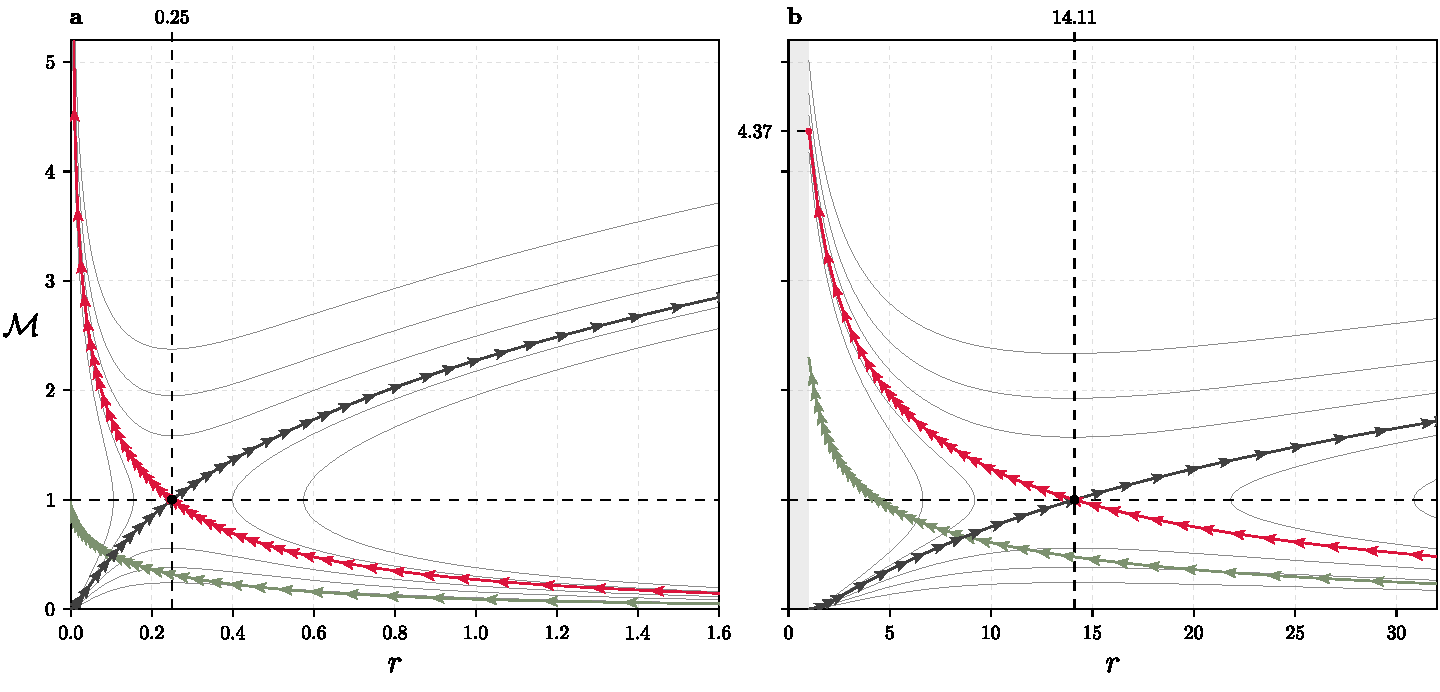
\includegraphics[width=\linewidth]{mach_topology.pdf}
\caption{Topology of the stationary solutions in the $(r,\mathcal{M})$ plane on linear axes: (a)~Bondi flow, Mach number $\mathcal{M}=v/a$, radius in units of the Bondi radius $r_{\mathrm{B}}=GM/a_{\infty}^{2}$; (b)~Michel flow at $a_{\infty}=0.1$, physical Mach number $\mathcal{M}=V/a$, where $V=|\upsilon|/\sqrt{f+\upsilon^{2}}$ is the speed measured by a locally static observer, radius in units of the gravitational radius $r_{\mathrm{g}}$. At a fixed Bernoulli integral every solution is a level line of the flux $\mathcal{J}$ ($r^{2}\rho v$ for Bondi, $r^{2}n\upsilon$ for Michel), so the whole family of solutions is the set of level lines of a single function $\mathcal{J}(r,\mathcal{M})$; the thin grey curves are the non-critical values $\mathcal{J}\neq\mathcal{J}_{\mathrm{c}}$. The critical flux at $\gamma=4/3$ corresponds to the pair of highlighted curves crossing at the sonic point: red is the accretion branch $\upsilon<0$, dark the wind branch $\upsilon>0$, with arrows showing the direction of the flow. The green curve is the critical accretion branch at $\gamma=5/3$, the second value used in this paper. The horizontal dashed line marks $\mathcal{M}=1$ and the vertical one the sonic point, whose radius is labelled on top ($0.25\,r_{\mathrm{B}}$ and $14.11\,r_{\mathrm{g}}$). The sonic point is the saddle of this family and the transonic solution its separatrix: the grey level lines either stay subsonic or supersonic throughout, reaching an extremum of the Mach number at the sonic point, or turn around at $\mathcal{M}=1$ without ever getting there. The inner boundaries of the two problems are of different nature, and on linear axes the difference is immediate. For Bondi the inner end lies at the centre itself, and the family splays apart there: the subsonic branches run into the origin as $\mathcal{M}\propto r^{(5-3\gamma)/[2(\gamma-1)]}$, while the supersonic ones hug the vertical axis and leave through the top of the frame as $\mathcal{M}\propto r^{(3\gamma-5)/4}$. Both exponents are proportional to $5-3\gamma$ and vanish at $\gamma=5/3$: the green curve in panel~(a) is subsonic at every finite radius and reaches $\mathcal{M}=1$ only at the point $r=0$ itself, to which the sonic point $r_{\mathrm{s}}=(5-3\gamma)r_{\mathrm{B}}/4$ has shrunk, so that no X-shaped crossing is left at any finite radius. For Michel, by contrast, the domain terminates at the gravitational horizon (grey band $r<r_{\mathrm{g}}$), the supersonic branches arriving there at finite Mach numbers: for the red branch it is $\mathcal{M}=4.37$, marked on the ordinate axis. Changing the adiabatic index breaks nothing here: the green branch at $\gamma=5/3$ is merely shifted inward along with the acoustic horizon ($r_{\mathrm{a}}=4.38\,r_{\mathrm{g}}$ instead of $14.11\,r_{\mathrm{g}}$) and terminates at the horizon at $\mathcal{M}=2.30$. The acoustic horizon stays at a finite radius for every $\gamma$, and this is exactly what sets the relativistic problem apart from the Newtonian one.}
\label{fig:mach_topology}
\end{figure}

As in the Michel problem, what diverges is not the potential but the physical fields reconstructed from its derivatives -- with the difference that the exponents are now nonzero. The radial response remains bounded,
\begin{equation}
    \ell=0:
    \quad
    \frac{\delta\rho}{\rho}
    \longrightarrow\mathrm{const},
    \qquad
    \frac{\delta v_{\mathrm{rad}}}{a}
    \sim r^{(5-3\gamma)/4},
    \label{eq:acoustic_critical_radial}
\end{equation}
whereas the non-radial one grows without limit:
\begin{equation}
    \ell\neq0:
    \quad
    \frac{\delta\rho}{\rho}
    \sim r^{-1/2},
    \qquad
    \frac{\delta v_{\mathrm{rad}}}{a}
    \sim r^{(3-3\gamma)/4},
    \qquad
    \frac{\delta v_{\mathrm{pol}}}{a}
    \sim r^{(3\gamma-7)/4}.
    \label{eq:acoustic_critical_nonradial}
\end{equation}
For $1<\gamma<5/3$ all three exponents in Eq.~\eqref{eq:acoustic_critical_nonradial} are negative, while at $\gamma=5/3$ the supersonic background asymptotics~\eqref{eq:bondi_freefall_asymptotics} themselves cease to hold: the central Mach number only approaches unity, as the green curve in Fig.~\ref{fig:mach_topology}(a) shows.

\subsection{Spatial stability and horizon regularization}
\label{sec:acoustic_stability}

Spatial instability at fixed real frequency is defined in Ref.~\cite{KovalenkoIG_EreminMA_SpatialInstabilityOfSphericalAccretion_1998} as unbounded growth of a perturbation relative to the background as it approaches the accretor. In the point-mass Bondi problem the solution domain extends to the singularity at $r=0$, and by the asymptotics~\eqref{eq:acoustic_critical_radial} and~\eqref{eq:acoustic_critical_nonradial} purely radial perturbations remain bounded, whereas non-radial ones grow without limit for $\gamma<5/3$ -- provided that the accretor is sufficiently small compared with the Bondi radius, $r_{\mathrm{acc}}\ll r_{\mathrm{B}}$.

In the Michel flow the domain is arranged differently. A perturbation arriving from infinity meets not a point singularity but the acoustic horizon $r_{\mathrm{a}}$, which serves as the inner boundary. By Eq.~\eqref{eq:michel_acoustic_horizon_asymptotics}, under the physical boundary condition all relative amplitudes approach finite values there, and they do so independently of $\ell$: the centrifugal part of the effective potential vanishes at the horizon, so no singular amplification arises at the inner boundary.

This yields a precise statement about the exterior domain: an acoustic perturbation arriving from infinity has a regular scattering solution throughout $r_{\mathrm{a}}\le r<\infty$, and the central power-law mechanism of the Newtonian problem is simply absent there. A disturbance created in the supersonic shell $1<r<r_{\mathrm{a}}$, in turn, is causally unable to return outward through the acoustic horizon at $r=r_{\mathrm{a}}$. This removal of the Newtonian singularity, together with its causal isolation, is what we call \emph{horizon regularization} of the spatial problem. The result complements the temporal-stability and quasi-normal analyses carried out in Refs.~\cite{MoncriefV_StabilityOfStationarySphericalAccretionOntoASchwarzschildBlackHole_1980,ChaverraE_MoralesMD_SarbachO_QuasinormalAcousticOscillationsInTheMichelFlow_2015}: the same exterior domain is confronted here with the spatial criterion set out in Ref.~\cite{KovalenkoIG_EreminMA_SpatialInstabilityOfSphericalAccretion_1998}.

This statement should not be confused either with a proof that all perturbations remain bounded down to the gravitational horizon, or with a general proof of temporal mode stability. The former would require a horizon-penetrating, freely falling description of the supersonic region, the latter an energy estimate or a complex-frequency analysis; both lie outside the spatial scattering problem considered here. Nor is the protection uniform in $a_{\infty}$: as $a_{\infty}\rightarrow0$ the horizon recedes, $r_{\mathrm{a}}\rightarrow\infty$, the exterior domain expands into the Newtonian regime, and the point-mass spatial problem is recovered. In the same way, if $r_{\mathrm{g}}$ is switched off, the inner boundary disappears along with the horizon, and the problem is once again closed by the singularity of Eq.~\eqref{eq:kovalenko_eremin_limit}.

\subsection{Acoustic scattering}
\label{sec:acoustic_numerics}

To check the exterior construction in practice, we integrate the Schr\"odinger equation~\eqref{eq:schrodinger_equation} numerically outward, starting from the acoustic horizon. The initial condition is a purely ingoing wave~\eqref{eq:horizon_boundary_condition}. At large $r_{*}$ the resulting solution is matched to a superposition of incident and reflected waves, from which the reflection and transmission amplitudes $R$ and $T$ are extracted:
\begin{equation}
    X
    \sim
    e^{-i\omega r_{*}}
    +R\,e^{i\omega r_{*}},
    \qquad
    r_{*}\rightarrow+\infty,
    \label{eq:scattering_amplitudes}
\end{equation}
while at the horizon itself
\begin{equation}
    X
    \sim
    T\,e^{-i\omega r_{*}},
    \qquad
    r_{*}\rightarrow-\infty.
    \label{eq:scattering_horizon_amplitude}
\end{equation}
Because the effective potential is real, Eq.~\eqref{eq:schrodinger_equation} implies conservation of flux. The associated Wronskian
\begin{equation}
    \mathcal{W}
    =
    \frac{1}{2i}
    \left(
        X^{*}\frac{\mathrm{d}X}{\mathrm{d}r_{*}}
        -
        X\frac{\mathrm{d}X^{*}}{\mathrm{d}r_{*}}
    \right)
    \label{eq:wronskian_flux}
\end{equation}
is constant throughout the exterior domain. Matching its values at the horizon and at infinity yields an exact relation between the scattering amplitudes:
\begin{equation}
    |R|^{2}+|T|^{2}=1.
    \label{eq:flux_conservation}
\end{equation}
This identity serves both as a physical check of the one-dimensional problem and as a control on the numerical accuracy of the integration.

Illustrative results for $a_{\infty}=0.1$ are collected in Table~\ref{tab:acoustic_scattering}. The corresponding acoustic horizons are $r_{\mathrm{a}}=4.38$ for $\gamma=5/3$ and $r_{\mathrm{a}}=14.11$ for $\gamma=4/3$. In the sampled cases the effective potential forms a finite barrier that vanishes at both asymptotic ends, so the scattering is fully described by the pair of coefficients $R$ and $T$.
\begin{table}[ht]
\centering
\caption{Illustrative acoustic scattering coefficients for
$a_{\infty}=0.1$.}
\label{tab:acoustic_scattering}
\begin{tabular}{ccccc}
\toprule
$\gamma$ & $\ell$ & $\omega$ & $|R|^{2}$ & $|T|^{2}$ \\
\midrule
$5/3$ & $1$ & $0.05$ & $0.003$ & $0.997$ \\
$5/3$ & $1$ & $0.20$ & $0.000$ & $1.000$ \\
$5/3$ & $2$ & $0.05$ & $0.439$ & $0.561$ \\
$5/3$ & $2$ & $0.20$ & $0.000$ & $1.000$ \\
$4/3$ & $1$ & $0.01$ & $0.040$ & $0.960$ \\
$4/3$ & $1$ & $0.04$ & $0.000$ & $1.000$ \\
$4/3$ & $2$ & $0.01$ & $0.487$ & $0.513$ \\
$4/3$ & $2$ & $0.04$ & $0.000$ & $1.000$ \\
\bottomrule
\end{tabular}
\end{table}

The absence of $|R|>1$ is expected for this static, real one-dimensional problem and confirms that the numerical implementation is sound; it is not, by itself, a proof against complex-frequency instabilities. Likewise, positivity of the sampled potentials supports the exterior stability picture only over the tested parameters. A systematic parameter survey and a direct comparison with the quasi-normal spectrum obtained in Ref.~\cite{ChaverraE_MoralesMD_SarbachO_QuasinormalAcousticOscillationsInTheMichelFlow_2015} lie beyond the scope of the present real-frequency spatial analysis and will be taken up separately in future work.

\section{Vortical modes}
\label{sec:vortical}

\subsection{Frozen-in vorticity}
\label{sec:frozen_vorticity}

We now turn to isentropic perturbations that carry vorticity: $\delta S=0$ and $\delta\omega_{\mu\nu}\neq0$. For these the linearized Euler equation~\eqref{eq:linearized_euler} reduces to the condition $u^{\mu}\delta\omega_{\mu\nu}=0$ of Eq.~\eqref{eq:vortex_frozen}, so the vorticity has no component along the flow. In the language of differential forms this is written $i_{u}\delta\omega=0$, where $i_{u}$ is the interior product with the four-velocity, $(i_{u}\delta\omega)_{\nu}=u^{\mu}\delta\omega_{\mu\nu}$. In addition, the vorticity is built from the one-form $w_{\mu}$ as $\delta\omega=\mathrm{d}w$, and any such form satisfies $\mathrm{d}\delta\omega=0$. Cartan's identity combines both properties:
\begin{equation}
    \mathcal{L}_{u}\delta\omega
    =
    i_{u}\mathrm{d}\delta\omega
    +
    \mathrm{d}(i_{u}\delta\omega)
    =0.
    \label{eq:vorticity_lie_dragged}
\end{equation}
Thus the flow carries the vorticity unchanged -- the relativistic Helmholtz--Kelvin theorem. What is conserved is the Lie transport of the two-form, not the individual components: gradients of $u^{\mu}$ stretch and compress the fluid element, so the radial amplitudes still vary.

For a stationary radial background the transport can be integrated. Every harmonic perturbation then carries the same advective phase
\begin{equation}
    \mathcal{P}_{\mathrm{v}}(r)
    =
    \exp\left(
        i\omega\int^{r}\frac{u^{t}}{u^{r}}\,\mathrm{d}r'
    \right)
    =
    \exp\left(
        i\omega\int^{r}\frac{\vartheta}{\upsilon}\,\mathrm{d}r'
    \right).
    \label{eq:vortex_advection_phase}
\end{equation}
The radial factors left after the phase is factored out merely record the stretching and compression of the flow tube. Two independent polarizations survive on the sphere. For $\ell=0$ nothing remains: spherical symmetry allows only the component $\delta\omega_{tr}$, and Eq.~\eqref{eq:vortex_frozen} sets it to zero.

Although $\delta\omega$ itself is transported autonomously, the observable perturbation is not. For $\delta S=0$, Eq.~\eqref{eq:perturbed_momentum} expresses the enthalpy and velocity in terms of $w_{\mu}$:
\begin{equation}
    \delta h
    =
    -u^{\mu}w_{\mu},
    \qquad
    h\,\delta u_{\mu}
    =
    \bigl(\delta_{\mu}^{\nu}+u_{\mu}u^{\nu}\bigr)w_{\nu}.
    \label{eq:vortical_enthalpy_velocity}
\end{equation}
Splitting $w_{\mu}$ into potential and vortical parts, $w_{\mu}=\partial_{\mu}\delta\varphi+w_{\mu}^{\perp}$, and substituting into the continuity equation yields the forced acoustic equation
\begin{equation}
    \nabla_{\mu}
    \left(
        \Omega^{2}\eta^{\mu\nu}
        \partial_{\nu}\delta\varphi
    \right)
    =
    -
    \nabla_{\mu}
    \left(
        \Omega^{2}\eta^{\mu\nu}w_{\nu}^{\perp}
    \right).
    \label{eq:vortical_forced_wave}
\end{equation}
Thus the advected invariant is the vorticity $\delta\omega_{\mu\nu}$, while the sound it produces is a forced response: in an inhomogeneous background ($\nabla_{\mu}u_{\nu}\neq0$) the vortical part $w_{\mu}^{\perp}$ acts as a source on the right-hand side of~\eqref{eq:vortical_forced_wave}. Let us now see where this transport takes the perturbation on the Michel background.

\subsection{Advection across the acoustic horizon}
\label{sec:vortical_transport}

The characteristics of Eq.~\eqref{eq:vorticity_lie_dragged} are the fluid worldlines. Their Schwarzschild-coordinate velocity is
\begin{equation}
    \left(\frac{\mathrm{d}r}{\mathrm{d}t}\right)_{\mathrm{v}}
    =
    \frac{u^{r}}{u^{t}}
    =
    \frac{\upsilon}{\vartheta}
    =
    -Vf<0,
    \label{eq:vortex_characteristic}
\end{equation}
where $V=-\upsilon/\sqrt{f+\upsilon^{2}}$ is the inward physical speed. The vorticity therefore has a single material characteristic, directed inward everywhere: unlike sound, it has no counter-propagating branch. A vortex created outside the acoustic horizon is carried by the flow across it, while vorticity already inside the supersonic shell $1<r<r_{\mathrm{a}}$ can never return to the exterior. Figure~\ref{fig:causal_structure}(b) shows the contrast directly: the fluid worldlines (black) cross the horizon inward from any emission radius, whereas the outgoing sound branch freezes there.

The Michel background and the flow map it generates are smooth at $r=r_{\mathrm{a}}>1$: the integrand $\vartheta/\upsilon$ in Eq.~\eqref{eq:vortex_advection_phase} is finite because $\upsilon_{\mathrm{a}}\neq0$, and for real $\omega$ the phase itself has unit modulus. Equation~\eqref{eq:vorticity_lie_dragged} therefore produces no power-law singularity at the horizon, and together with the forced response the relative amplitudes approach finite values:
\begin{equation}
    \frac{\delta n}{n},\
    \frac{\delta v_{\mathrm{rad}}}{a},\
    \frac{\delta v_{\mathrm{pol}}}{a},\
    \frac{\delta v_{\mathrm{tor}}}{a}
    \sim x^{0},
    \qquad
    r \rightarrow r_{\mathrm{a}}.
    \label{eq:michel_vortex_horizon_asymptotics}
\end{equation}
The forced potential response~\eqref{eq:vortical_forced_wave} does involve both acoustic characteristics, but its source is regular, and with a regular source the exterior wave problem is regular as well (Sec.~\ref{sec:boundary_asymptotics}).

Schwarzschild coordinates alone, however, do not establish that every physical vorticity component stays bounded all the way to the gravitational horizon: there $\mathrm{d}r/\mathrm{d}t\rightarrow0$ and the phase in Eq.~\eqref{eq:vortex_advection_phase} acquires the usual coordinate singularity. Determining the amplitudes in the freely falling frame inside the acoustic horizon requires a horizon-penetrating analysis. Nor is the regularization uniform in the cold limit: as $a_{\infty}\rightarrow0$ the horizon recedes to infinity, $r_{\mathrm{a}}\rightarrow\infty$, leaving a parametrically large Newtonian region in which relative vortical amplitudes can grow before it is reached.

\subsection{Newtonian limit and Bondi asymptotics}
\label{sec:newtonian_bondi_vortical}

How much the replacement of the center by a horizon matters is seen in the Newtonian limit~\eqref{eq:newtonian_limit}. With $w_{i}\rightarrow\delta v_{i}$, the spatial components of the two-form~\eqref{eq:perturbed_momentum} become
\begin{equation}
    \delta\omega_{ij}
    =
    \partial_{i}\delta v_{j}
    -
    \partial_{j}\delta v_{i},
    \label{eq:vorticity_newtonian_components}
\end{equation}
and in three-dimensional Euclidean space one associates to this two-form the Hodge-dual vorticity vector
\begin{equation}
    \delta q^{k}
    =
    \tfrac{1}{2}\varepsilon^{kij}\delta\omega_{ij}
    =
    \bigl(\boldsymbol{\nabla}\times\delta\boldsymbol{v}\bigr)^{k}
    \quad\to\quad
    \delta\boldsymbol{q}
    =
    \boldsymbol{\nabla}\times\delta\boldsymbol{v}.
    \label{eq:vorticity_newtonian}
\end{equation}
Here $\delta\boldsymbol{q}$ is the vorticity vector of the perturbation and $\boldsymbol{v}$ is the background flow velocity. Equation~\eqref{eq:vorticity_lie_dragged} then becomes
\begin{equation}
    \partial_{t}\delta\boldsymbol{q}
    +
    (\boldsymbol{v}\boldsymbol{\cdot}\boldsymbol{\nabla})
        \delta\boldsymbol{q}
    -
    (\delta\boldsymbol{q}\boldsymbol{\cdot}\boldsymbol{\nabla})
        \boldsymbol{v}
    +
    \delta\boldsymbol{q}\,
        (\boldsymbol{\nabla}\boldsymbol{\cdot}\boldsymbol{v})
    =0.
    \label{eq:vorticity_transport_vector}
\end{equation}
For a radial background $\boldsymbol{v}=\upsilon\,\boldsymbol{e}_{r}$, Eq.~\eqref{eq:vorticity_transport_vector} coincides with the vorticity equation of Ref.~\cite{KovalenkoIG_EreminMA_SpatialInstabilityOfSphericalAccretion_1998}, so all Bondi-flow consequences that follow from it are already given there.

The main one is the behavior of the amplitudes near the center. With the free-fall asymptotics~\eqref{eq:bondi_freefall_asymptotics}, each of the two non-radial polarizations acquires a diverging response. The polarization with radial vorticity perturbs neither the density nor the compressible part of the velocity, and only its toroidal amplitude grows,
\begin{equation}
    \delta q_{r}\neq0:
    \quad
    \frac{\delta v_{\mathrm{tor}}}{a}
    \sim r^{(3\gamma-7)/4},
    \label{eq:vortex_critical_toroidal}
\end{equation}
whereas for the polarization without radial vorticity the growing quantities are the same as in the acoustic sector:
\begin{equation}
    \delta q_{r}=0:
    \quad
    \frac{\delta\rho}{\rho}
    \sim r^{-1/2},
    \qquad
    \frac{\delta v_{\mathrm{rad}}}{a}
    \sim r^{(3-3\gamma)/4},
    \qquad
    \frac{\delta v_{\mathrm{pol}}}{a}
    \sim r^{(3\gamma-7)/4}.
    \label{eq:vortex_critical_asymptotics}
\end{equation}
All of these exponents are negative for $1<\gamma\leq5/3$, whereas for $\ell=0$ the vorticity vanishes identically and there is nothing to grow. The central divergence~\eqref{eq:vortex_critical_toroidal}--\eqref{eq:vortex_critical_asymptotics} thus belongs to the $r\rightarrow0$ asymptotics, which the exterior Michel domain simply does not contain: there every exponent vanishes, Eq.~\eqref{eq:michel_vortex_horizon_asymptotics}.

\section{Entropy modes and mode coupling}
\label{sec:entropy}

\subsection{Entropy advection}
\label{sec:entropy_advection}

An entropy perturbation is a scalar inhomogeneity attached to a fluid element. Unlike vorticity, it has no tensorial structure and hence no geometric compression factors: what is transported is the scalar itself. On a stationary radial background, Eq.~\eqref{eq:entropy_mode_advection} for a single harmonic reduces to
\begin{equation}
    \left(
        -i\omega u^{t}+u^{r}\frac{\mathrm{d}}{\mathrm{d}r}
    \right)\widetilde{S}_{\ell m}=0
\end{equation}
and is solved by the same advective phase~\eqref{eq:vortex_advection_phase} as in the vortical sector:
\begin{equation}
    \delta S
    =
    \widetilde{S}_{\ell m}(r)
    Y_{\ell m}(\theta,\phi)e^{-i\omega t},
    \qquad
    \widetilde{S}_{\ell m}(r)
    =
    S_{\ell m}\,
    \mathcal{P}_{\mathrm{v}}(r).
    \label{eq:entropy_advection_solution}
\end{equation}
The amplitude $S_{\ell m}$ stays constant along the streamlines, so entropy and vorticity ride the same material characteristic and differ only in the fields they force.

For the normalization $S=\ln K$ adopted in Sec.~\ref{sec:linearized_system}, the polytropic equation of state relates it to the pressure and density perturbations:
\begin{equation}
    \delta S
    =
    \frac{\delta p}{p}
    -
    \gamma\frac{\delta n}{n}.
    \label{eq:entropy_thermodynamic_definition}
\end{equation}
The scalar itself is unchanged by the transport, whereas the density and velocity perturbations accompanying it are fixed by the forced response, to which we now turn.

\subsection{Baroclinic excitation of sound and vorticity}
\label{sec:mode_coupling}

The forced response begins with the density. The thermodynamic relation~\eqref{eq:thermodynamic_perturbation} already derived becomes, for $S=\ln K$,
\begin{equation}
    \delta n
    =
    \frac{n}{ha^{2}}\,\delta h
    -
    \frac{n}{\gamma-1}\,\delta S.
    \label{eq:entropy_density_split}
\end{equation}
The first term is the variation at fixed entropy; the second is the contribution of $\delta S$ itself at fixed enthalpy. These should not be read as two independently evolving density fields: the Euler equation couples the associated momentum response.

The coupling is most transparent in the language of differential forms. Taking the exterior derivative of Eq.~\eqref{eq:entropy_vorticity_source} and using $\mathrm{d}\delta\omega=0$ together with the Cartan identity~\eqref{eq:vorticity_lie_dragged} gives
\begin{equation}
    \mathcal{L}_{u}\delta\omega
    =
    \mathrm{d}T\wedge\mathrm{d}\delta S,
    \label{eq:entropy_baroclinic_vorticity}
\end{equation}
where $\mathcal{L}_{u}$ is the Lie derivative along the background flow and $\wedge$ the antisymmetric exterior product. The right-hand side is the relativistic baroclinic source: vorticity is generated wherever the gradients of temperature and entropy fail to be parallel. On a spherical background $\mathrm{d}T$ is radial, so the rotational part of the source is nonzero only for $\ell\neq0$, when $\mathrm{d}\delta S$ has an angular component. A purely radial entropy perturbation can force compression, but it cannot generate spatial vorticity.

The acoustic link proceeds through the same momentum decomposition $w_{\mu}=\partial_{\mu}\delta\varphi+w_{\mu}^{\perp}$ and the same relations~\eqref{eq:vortical_enthalpy_velocity} as in the vortical sector. The continuity equation now gives
\begin{equation}
    \nabla_{\mu}
    \left(
        \Omega^{2}\eta^{\mu\nu}\partial_{\nu}\delta\varphi
    \right)
    =
    -
    \nabla_{\mu}
    \left(
        \Omega^{2}\eta^{\mu\nu}w_{\nu}^{\perp}
    \right)
    -
    \nabla_{\mu}
    \left(
        n\chi u^{\mu}\delta S
    \right).
    \label{eq:entropy_forced_wave_general}
\end{equation}
For the present polytrope $\chi=-(\gamma-1)^{-1}$ is constant, and baryon conservation together with entropy advection makes the last term vanish identically, $\nabla_{\mu}(n\chi u^{\mu}\delta S)=0$. There is thus no direct scalar source of $\delta S$ in the continuity equation: entropy excites sound only indirectly, through the nonexact momentum $w_{\mu}^{\perp}$ generated by Eq.~\eqref{eq:entropy_vorticity_source}. Equations~\eqref{eq:entropy_advection_solution}, \eqref{eq:entropy_vorticity_source}, and~\eqref{eq:entropy_forced_wave_general} therefore form a triangular system: entropy is advected autonomously, while the vortical and acoustic fields are forced by it.

Let us now follow that system down to the acoustic horizon. Equation~\eqref{eq:entropy_advection_solution} has the same single inward characteristic as Eq.~\eqref{eq:vortex_characteristic}: an entropy inhomogeneity crosses the horizon with the fluid and has no independent outgoing branch. While it remains outside, it does emit an acoustic response, so what removes the Newtonian central instability here is not causality but the regularity of the coupled exterior problem. The Michel background, the advected scalar $\delta S\rightarrow S_{\ell m}\mathcal{P}_{\mathrm{v}}(r_{\mathrm{a}})$, and the baroclinic source $\mathrm{d}T\wedge\mathrm{d}\delta S$ are smooth at $r=r_{\mathrm{a}}$, and Eq.~\eqref{eq:entropy_forced_wave_general} is the regular exterior acoustic equation with a regular source. At the horizon, therefore,
\begin{equation}
    \ell=0:
    \quad
    \frac{\delta n}{n},\
    \frac{\delta v_{\mathrm{rad}}}{a}
    \sim x^{0};
    \qquad
    \ell\neq0:
    \quad
    \frac{\delta n}{n},\
    \frac{\delta v_{\mathrm{rad}}}{a},\
    \frac{\delta v_{\mathrm{pol}}}{a}
    \sim x^{0},
    \qquad
    r \rightarrow r_{\mathrm{a}},
    \label{eq:michel_entropy_horizon_asymptotics}
\end{equation}
and the distinction between the radial and non-radial cases disappears at the horizon together with the angular barrier.

This statement does not rely on a presumed large-enthalpy suppression near the horizon; no such suppression is generic for Michel flow. As in the vortical sector, the cold limit is nonuniform: when $a_{\infty}\rightarrow0$ and $r_{\mathrm{a}}\rightarrow\infty$, the extended Newtonian region can produce substantial forced amplitudes before the perturbation reaches the acoustic horizon.

\subsection{Newtonian limit and Bondi asymptotics}
\label{sec:newtonian_bondi_entropy}

In the Newtonian limit~\eqref{eq:newtonian_limit} the entropy sector reduces to
\begin{equation}
    \frac{D\delta S}{Dt}=0,
    \qquad
    \frac{D\delta\rho}{Dt}
    +\delta\rho\,\boldsymbol{\nabla}\boldsymbol{\cdot}\boldsymbol{v}
    +\boldsymbol{\nabla}\boldsymbol{\cdot}
        (\rho\delta\boldsymbol{v})=0,
    \label{eq:entropy_newtonian_continuity}
\end{equation}
\begin{equation}
    \frac{D\delta\boldsymbol{v}}{Dt}
    +
    (\delta\boldsymbol{v}\boldsymbol{\cdot}\boldsymbol{\nabla})
        \boldsymbol{v}
    =
    -\frac{1}{\rho}\boldsymbol{\nabla}\delta p
    +\frac{\delta\rho}{\rho^{2}}\boldsymbol{\nabla}p,
    \qquad
    \delta p=a^{2}\delta\rho+p\delta S,
    \label{eq:entropy_newtonian_euler}
\end{equation}
where $D/Dt=\partial_{t}+\boldsymbol{v}\boldsymbol{\cdot}\boldsymbol{\nabla}$ is the derivative along the unperturbed flow. After spherical harmonic decomposition this system coincides with the entropy-perturbation system of Ref.~\cite{KovalenkoIG_EreminMA_SpatialInstabilityOfSphericalAccretion_1998}, while the entropy itself retains the amplitude $S_{\ell m}$ and the Newtonian limit of the phase in Eq.~\eqref{eq:entropy_advection_solution}.

The main consequences appear in the central asymptotics of the forced response. For the critical supersonic Bondi flow, Eq.~\eqref{eq:bondi_freefall_asymptotics} gives
\begin{equation}
    \ell=0:
    \quad
    \frac{\delta\rho}{\rho}
    \sim r^{(5-3\gamma)/2},
    \qquad
    \frac{\delta v_{\mathrm{rad}}}{a}
    \sim r^{(5-3\gamma)/4},
    \label{eq:entropy_critical_radial}
\end{equation}
whereas for $\ell\neq0$,
\begin{equation}
    \frac{\delta\rho}{\rho}
    \longrightarrow-\frac{S_{\ell m}}{\gamma},
    \qquad
    \frac{\delta v_{\mathrm{rad}}}{a}
    \sim r^{(5-3\gamma)/4},
    \qquad
    \frac{\delta v_{\mathrm{pol}}}{a}
    \sim r^{3(5-3\gamma)/4}.
    \label{eq:entropy_critical_nonradial}
\end{equation}
All exponents are nonnegative for $1<\gamma\leq5/3$, so in the critical flow the entropy-forced response stays finite: of the three sectors, this is the only one free of a central divergence there. In a subcritical flow the radial response is finite as well, but the polar velocity grows: $\delta v_{\mathrm{pol}}/a\sim r^{-3/2}$ for $1<\gamma<4/3$ and $\sim r^{(3\gamma-5)/[2(\gamma-1)]}$ for $4/3<\gamma<5/3$. This reproduces the distinction between critical and subcritical accretion established in Ref.~\cite{KovalenkoIG_EreminMA_SpatialInstabilityOfSphericalAccretion_1998} -- a distinction that on the Michel background is smoothed into the common vanishing exponents~\eqref{eq:michel_entropy_horizon_asymptotics}.

\section{Unified spectrum and discussion}
\label{sec:discussion}

\subsection{Mode classification and stability summary}
\label{sec:unified_classification}

The three families are distinguished most sharply by their characteristics. Free acoustic perturbations have two branches and propagate on the null cone of the acoustic metric. Vorticity and entropy each have one material characteristic, tangent to the background 4-velocity. In an inhomogeneous flow, however, this kinematic classification does not diagonalize the complete perturbation problem: advected vorticity forces a potential response, while entropy first generates non-exact momentum through the baroclinic term and thereby forces both vorticity and sound. The resulting hierarchy is triangular,
\begin{equation}
    \delta S
    \longrightarrow
    w_{\mu}^{\perp}
    \longrightarrow
    \delta\varphi,
    \qquad
    \delta\omega_{\mu\nu}^{\mathrm{free}}
    \longrightarrow
    w_{\mu}^{\perp}
    \longrightarrow
    \delta\varphi,
    \label{eq:mode_coupling_hierarchy}
\end{equation}
with no linear feedback from the forced acoustic field into the advected invariant $\delta S$. The first arrow includes the entropy-generated vorticity described by Eq.~\eqref{eq:entropy_baroclinic_vorticity}.

Table~\ref{tab:mode_stability_summary} separates the Newtonian central asymptotics from the exterior relativistic result. Here ``regular'' means specifically that the solution has no Newtonian $r\rightarrow0$ power-law divergence in $r\geq r_{\mathrm{a}}$; it is not a claim about arbitrary complex-frequency modes or about freely falling amplitudes inside the acoustic horizon.

\begin{table}[ht]
\centering
\caption{Characteristics and spatial behaviour of the three perturbation families. The Newtonian column refers to the $r\rightarrow0$ asymptotics of Bondi flow; the relativistic column refers only to the exterior Michel domain.}
\label{tab:mode_stability_summary}
\small
\setlength{\tabcolsep}{4pt}
\renewcommand{\arraystretch}{1.15}
\begin{tabular}{
    >{\raggedright\arraybackslash}p{2.8cm}
    >{\raggedright\arraybackslash}p{2.5cm}
    >{\raggedright\arraybackslash}p{4.8cm}
    >{\raggedright\arraybackslash}p{4.7cm}}
\toprule
Family & Characteristic & Newtonian central behaviour & Exterior Michel domain \\
\midrule
Acoustic & two acoustic branches & finite for $\ell=0$; grows for $\ell\neq0$ when $\gamma<5/3$ & ingoing condition at $r_{\mathrm{a}}$; vanishing exponents~\eqref{eq:michel_acoustic_horizon_asymptotics} \\
Vortical & one material branch & absent for $\ell=0$; grows for $\ell\neq0$ throughout $1<\gamma\leq5/3$ & invariant advected inward; vanishing exponents~\eqref{eq:michel_vortex_horizon_asymptotics} \\
Entropy & one material branch & finite in critical flow; subcritical non-radial response grows for $\gamma<5/3$ & scalar invariant advected inward; vanishing exponents~\eqref{eq:michel_entropy_horizon_asymptotics} \\
\bottomrule
\end{tabular}
\end{table}

The common relativistic statement is therefore narrower, but also cleaner, than a blanket assertion of stability. The physical Michel solution supplies a regular acoustic-horizon boundary at a finite radius and causally isolates the supersonic shell. The homogeneous acoustic problem is regular there, and regular vortical or entropy data provide regular sources for it. Thus the central endpoint responsible for the Bondi power laws is absent from the externally accessible boundary-value problem for all three sectors. This conclusion complements, rather than replaces, temporal energy estimates and quasi-normal-mode analyses.

\subsection{Dependence on the equation of state}
\label{sec:parameter_dependence}

The equation of state enters the spectrum along two different routes. First, the index $\gamma$ governs the Newtonian power laws by which central growth is diagnosed: the radial acoustic exponent~\eqref{eq:acoustic_critical_radial} vanishes at $\gamma=5/3$, where the supersonic background asymptotics~\eqref{eq:bondi_freefall_asymptotics} themselves also cease to hold; the non-radial acoustic and vortical exponents are negative throughout $1<\gamma\leq5/3$; the entropy response of the critical flow, by contrast, stays finite across that whole interval. Second, the pair $(\gamma,a_{\infty})$ already fixes the entire Michel background, and with it the location of the acoustic horizon, the acoustic tortoise coordinate, and both terms of the effective potential~\eqref{eq:effective_potential}. These wave quantities cannot be inferred from the Newtonian exponents alone.

The distinction is visible in the two backgrounds of Sec.~\ref{sec:acoustic_numerics}. At $a_{\infty}=0.1$ the horizon of the $\gamma=5/3$ flow sits at $r_{\mathrm{a}}=4.38$, whereas for $\gamma=4/3$ it lies three times farther out, at $r_{\mathrm{a}}=14.11$; nevertheless, in both cases the effective potential forms a finite barrier, the flux is conserved, and $|R|^{2}\leq1$. Increasing $\ell$ strengthens the centrifugal part of the barrier and raises the low-frequency reflection, while modes with $\omega^{2}$ well above the barrier maximum are transmitted almost without reflection. The frequencies in Table~\ref{tab:acoustic_scattering} are chosen on the scale of each background separately, so they verify each scattering problem but do not yet constitute a controlled comparison of reflection as a function of $\gamma$.

What does not depend on the parameters is the conclusion about the regularity of the inner boundary: it holds for every transonic Michel solution with finite $r_{\mathrm{a}}$. The quantitative amplification of a perturbation before horizon crossing is a separate question, set by the full radial profiles rather than by $r_{\mathrm{a}}$ alone; in particular, both the limit $a_{\infty}\rightarrow0$ and the removal of the gravitational radius are singular limits of the comparison with Bondi flow. A systematic map of barrier heights, forced responses, and scattering coefficients over the $(\gamma,a_{\infty})$ plane should therefore extend the calculation presented here, rather than follow from it automatically.

\subsection{Relation to geometric optics}
\label{sec:geometric_optics_limit}

The high-frequency limit ties the wave problem to the ray picture of the companion study~\cite{SemyannikovAV_AcousticGeometryAndSoundRayDynamics_2026}. The eikonal relation~\eqref{eq:acoustic_eikonal_relation}, derived in Sec.~\ref{sec:acoustic_wave_equation}, already identifies acoustic rays as the null bicharacteristics of that effective geometry. The barriers agree as well: for large $\ell$ the leading term of the effective potential~\eqref{eq:effective_potential} is
\begin{equation}
    V_{\mathrm{eff}}
    =
    \ell(\ell+1)U(r)+O(\ell^{0}),
    \qquad
    U(r)=\frac{a^{2}\eta^{rr}}{r^{2}},
    \label{eq:eikonal_capture_barrier}
\end{equation}
which is precisely the ray capture barrier whose maximum defines the acoustic photon sphere. The remaining term $\smash{W^{-1/2}\mathrm{d}^{2}\sqrt{W}/\mathrm{d}r_{*}^{2}}$ controls finite-frequency amplitudes and is subleading in the large angular-momentum limit. The wave and ray tortoise coordinates differ globally, but at the horizon they share the same logarithmic behaviour, governed by the same acoustic surface gravity.

The two advected families do not reduce to this null dynamics at any frequency. Their eikonal relation is instead
\begin{equation}
    u^{\mu}k_{\mu}=0,
    \label{eq:advected_eikonal_relation}
\end{equation}
so for any $\omega$ their characteristics remain fluid worldlines and their radial phase remains the factor $\mathcal{P}_{\mathrm{v}}$ of Eq.~\eqref{eq:vortex_advection_phase}; what propagates on the acoustic cone is only the sound emitted by their forced potential response. The high-frequency picture therefore contains two different causal structures: acoustic disturbances follow the null cone of the effective metric, whereas the vortical and entropy invariants are transported on the material congruence and feed the acoustic sector along the way.

\section{Conclusions}
\label{sec:conclusions}

We have carried the Newtonian spatial-stability analysis of spherical accretion~\cite{KovalenkoIG_EreminMA_SpatialInstabilityOfSphericalAccretion_1998} over to the relativistic Michel flow, treating the acoustic, vortical, and entropy sectors within a single acoustic-geometry framework. The linearized continuity, Lichnerowicz--Crocco, and entropy-advection equations separate the perturbations into a potential acoustic mode, two advected vortical modes, and one advected entropy mode, coupled in an inhomogeneous flow through the baroclinic term and the continuity equation.

The acoustic sector reduces to a one-dimensional Schr\"odinger equation with an explicit effective potential. Two independent limits validate the reduction: it recovers the scalar Schwarzschild potential in vacuum and the Newtonian wave equation of the Bondi problem~\cite{KovalenkoIG_EreminMA_SpatialInstabilityOfSphericalAccretion_1998} in the nonrelativistic limit. For the transonic background the sonic point coincides with the acoustic horizon, and a Frobenius analysis gives a purely imaginary non-trivial exponent there, so the local solutions are travelling waves rather than growing powers.

The central result is that the acoustic horizon regularizes the externally accessible spatial problem. The Newtonian non-radial instability relies on growth towards a point-mass endpoint, $r\rightarrow0$; the exterior Michel domain has no such endpoint: the relative amplitudes of all three sectors approach finite values at the horizon, and the supersonic shell $1<r<r_{\mathrm{a}}$ is causally disconnected from it. In the two advected sectors the mechanism is even more transparent: with a single ingoing characteristic, vorticity and entropy are frozen into the flow and swept below the horizon, while the entropy mode additionally sources sound and vorticity through a regular baroclinic term. Acoustic scattering confirms flux conservation and the absence of superradiance. The Newtonian central power-law instability is therefore an artifact of the point mass and does not survive its replacement by a black hole.

Two caveats delimit the scope of these statements. First, the result concerns exterior spatial regularity rather than a general proof of temporal mode stability: the latter would require an energy estimate or a complex-frequency analysis, just as establishing the freely falling amplitudes inside the acoustic horizon would require a horizon-penetrating description. Second, the protection is not uniform in the cold limit: as $a_{\infty}\rightarrow0$ the horizon recedes to infinity, $r_{\mathrm{a}}\rightarrow\infty$, and the Newtonian regime is recovered. Natural extensions of this work are a systematic survey of the $(\gamma,a_{\infty})$ plane with a direct comparison to the quasi-normal spectrum, and the inclusion of non-adiabatic flow, rotation, and perturbation backreaction on the background.

\clearpage

\bibliographystyle{elsarticle-num}
\bibliography{article}

\end{document}
